\chapter{각운동량 다중항, 방사 운동, 그리고 조화진동자의 사다리}

\section{파동함수의 각도 의존성}

중심력장 안의 입자는 방사 좌표 하나와 각좌표 둘로 위치가 정해진다. 고전역학에서는
\begin{equation}
\mathbf L=\mathbf r\times\mathbf p
\end{equation}
가 벡터로서 보존된다. 그 방향은 궤도면을 정하지만, 궤도가 원형일 필요는 없다.

양자역학에서는 입자를
\begin{equation}
\Psi=\Psi(r,\theta,\phi),
\end{equation}
로 기술하며, 각운동량은 이 파동함수의 각도 의존성과 관련된다.

2차원에서는 각운동량 성분이 하나뿐이며, 이는 평면에 수직인 축을 중심으로 한 회전의 생성자이다.
\begin{equation}
L_z=-i\hbar\frac{\partial}{\partial\theta}.
\end{equation}
고윳값이 \(\hbar\ell\)인 고유함수는 다음을 만족한다.
\begin{equation}
-i\hbar\frac{\partial}{\partial\theta}\psi(r,\theta)
=\hbar\ell\,\psi(r,\theta).
\end{equation}
좌표 \(r\)는 이 방정식에서 영향을 받지 않는다. 해는 다음 형태이다.
\begin{equation}
\psi(r,\theta)=\chi(r)e^{i\ell\theta}.
\end{equation}
통상적인 단일값 궤도 파동함수라면 \(\theta\to\theta+2\pi\) 후에도 같은 점으로 돌아와야 하므로 \(\ell\)는 정수여야 한다. 방사 인자 \(\chi(r)\)는 에너지에는 영향을 줄 수 있지만, 이 각운동량 고윳값에는 영향을 주지 않는다.

3차원에서 이에 대응하는 분리는 방사 의존성과 구면 위의 함수를 분리한다.
\begin{equation}
\Psi(r,\theta,\phi)=R(r)Y_{\ell m}(\theta,\phi).
\end{equation}
함수 \(Y_{\ell m}\)는 구면조화함수이다. 여기서는 그 명시적 공식을 사용할 필요가 없다. 회전은 각도 인자에 작용하고 방사 함수에는 작용하지 않는다.

\section{유한한 각운동량 다중항}

각운동량 성분들은 다음 교환 관계를 만족한다.
\begin{equation}
\begin{aligned}
[L_x,L_y]&=i\hbar L_z,\\
[L_y,L_z]&=i\hbar L_x,\\
[L_z,L_x]&=i\hbar L_y.
\end{aligned}
\end{equation}
\(L_z\)의 고유상태를 택하고,
\begin{equation}
L_z|\ell,m\rangle=\hbar m\,|\ell,m\rangle,
\end{equation}
다음을 정의하자.
\begin{equation}
L_\pm=L_x\pm iL_y.
\end{equation}
교환 관계
\begin{equation}
[L_z,L_\pm]=\pm\hbar L_\pm
\end{equation}
로부터 다음을 얻는다.
\begin{align}
L_z\bigl(L_\pm|\ell,m\rangle\bigr)
&=\bigl(L_\pm L_z+[L_z,L_\pm]\bigr)|\ell,m\rangle \\
&=\hbar(m\pm1)L_\pm|\ell,m\rangle.
\end{align}
따라서 \(L_+\)는 \(m\)를 1만큼 높이고, \(L_-\)는 1만큼 낮춘다. 단, 그 결과 벡터가 영벡터가 되는 경우는 예외이다.

유한한 다중항에는 최고 상태와 최저 상태가 있다.
\begin{equation}
L_+|\ell,\ell\rangle=0,
\qquad
L_-|\ell,-\ell\rangle=0.
\end{equation}
\(+z\) 방향과 \(-z\) 방향은 회전으로 서로 연결되므로, 유한한 스펙트럼은 0을 중심으로 대칭이다. 따라서 고윳값은 다음과 같다.
\begin{equation}
m=-\ell,-\ell+1,\ldots,\ell-1,\ell,
\end{equation}
상태의 수는
\begin{equation}
2\ell+1.
\end{equation}
이다. 이웃한 값들의 차이가 1이므로 양 끝값은 정수 또는 반정수일 수 있다. 통상적인 궤도 구면조화함수는 정수인 경우를 구현하며, 추상적인 각운동량 대수는 반정수 다중항도 허용한다.

\begin{classroomqa}\lecturetimestamp{00:16:12}\audiencequestion{각운동량 다중항에 무한히 많은 상태가 들어갈 수 있습니까?}\lecturerresponse{그 가능성을 생각해 볼 수는 있지만, 여기서는 다룰 필요가 없습니다. 다른 상태의 특성을 고정하면 각운동량은 대체로 에너지를 높이므로, 유한한 에너지 상태를 논할 때 무한한 각운동량을 갖는 상태는 관련이 없습니다.}\end{classroomqa}

\section{\texorpdfstring{\(L^2\)}{의 공통 고윳값}}

각운동량 크기의 제곱을 재는 연산자는
\begin{equation}
L^2=L_x^2+L_y^2+L_z^2.
\end{equation}
사다리 연산자들의 순서곱은
\begin{align}
L_-L_+
&=(L_x-iL_y)(L_x+iL_y) \\
&=L_x^2+L_y^2+i[L_x,L_y] \\
&=L_x^2+L_y^2-\hbar L_z.
\end{align}
이다. 따라서
\begin{equation}
L^2=L_z^2+\hbar L_z+L_-L_+.
\end{equation}
이 항등식을 최고 상태에 적용하자. \(L_+|\ell,\ell\rangle=0\)이므로,
\begin{align}
L^2|\ell,\ell\rangle
&=\left(L_z^2+\hbar L_z+L_-L_+\right)|\ell,\ell\rangle \\
&=\hbar^2\left(\ell^2+\ell\right)|\ell,\ell\rangle,
\end{align}
따라서
\begin{equation}
L^2|\ell,\ell\rangle
=\hbar^2\ell(\ell+1)|\ell,\ell\rangle.
\end{equation}
이다. 제곱 크기는 \(\hbar^2\ell^2\)가 아니다. 추가 항은 각운동량 성분들의 비가환성에서 비롯된다.

같은 고윳값은 최고 상태뿐 아니라 다중항의 모든 상태에 속한다.

\begin{classroomqa}\lecturetimestamp{00:26:08}\audiencequestion{다른 상태들도 같은 \(L^2\) 값을 갖는다는 것을 보이는 연습문제는 정확히 무엇을 하라는 것입니까?}\lecturerresponse{\(L^2\)가 각운동량의 모든 성분과, 따라서 \(L_-\)와도 교환함을 보이시오. 그런 다음 \(L^2\)를 \(L_-\) 너머로 교환하시오. 최고 상태의 고윳값이 \(\hbar^2\ell(\ell+1)\)라면 그다음 상태도 같은 고윳값을 갖는다. 이 논증을 반복하면 그 값이 사다리 전체에 걸쳐 유지됨을 보일 수 있다.}\end{classroomqa}

실제로,
\begin{equation}
[L^2,L_i]=0,
\qquad i=x,y,z,
\end{equation}
이므로
\begin{equation}
[L^2,L_\pm]=0.
\end{equation}
이다. 예를 들어,
\begin{align}
L^2\bigl(L_-|\ell,\ell\rangle\bigr)
&=L_-L^2|\ell,\ell\rangle \\
&=\hbar^2\ell(\ell+1)L_-|\ell,\ell\rangle.
\end{align}
아래쪽으로 계속 내려가면 다음을 얻는다.
\begin{equation}
L^2|\ell,m\rangle
=\hbar^2\ell(\ell+1)|\ell,m\rangle
\end{equation}
모든 \(m=-\ell,\ldots,\ell\)에 대해 성립한다.

반대 순서로 곱해도 동등한 인수분해를 얻는다.
\begin{align}
L_+L_-
&=(L_x+iL_y)(L_x-iL_y) \\
&=L_x^2+L_y^2-i[L_x,L_y] \\
&=L_x^2+L_y^2+\hbar L_z,
\end{align}
따라서
\begin{equation}
L^2=L_z^2-\hbar L_z+L_+L_-.
\end{equation}

\begin{classroomqa}\lecturetimestamp{00:32:05}\audiencequestion{\(L_+L_-\)를 사용해 \(L_x^2+L_y^2\)를 반대 순서로 인수분해할 수 있습니까?}\lecturerresponse{그렇습니다. \(L_z\) 항의 부호가 반대로 바뀝니다. 이 순서에서는 최고 상태 대신 최저 상태에 항등식을 적용합니다. 최저 상태는 \(L_-\)에 의해 영벡터로 보내집니다. 같은 고윳값 \(\hbar^2\ell(\ell+1)\)를 얻습니다.}\end{classroomqa}

따라서 구면조화함수는 다음을 만족한다.
\begin{align}
L^2Y_{\ell m}
&=\hbar^2\ell(\ell+1)Y_{\ell m}, \\
L_zY_{\ell m}
&=\hbar m\,Y_{\ell m}.
\end{align}
각 궤도 양자수 \(\ell=0,1,2,\ldots\)마다 \(2\ell+1\)개의 함수가 있으며, 이 함수들은 \(m=-\ell,\ldots,\ell\)로 표시된다.

중심 퍼텐셜에서는
\begin{equation}
[H,L_i]=0.
\end{equation}
방사 에너지 고유상태와 \(\ell\)를 고정하면, \(m\)를 바꾸어도 \(L_\pm\)에 따라 바뀌는 에너지는 없다. 따라서 각 방사 고유상태는 \(2\ell+1\)차원의 자기 양자수 다중항을 이룬다.

아래에는 정수 궤도 사다리를 나타냈다.\footnote{이 도식은 강의 영상 \(00{:}35{:}53\)에서 확인할 수 있는 다중항 스케치와 연산자 항등식을 바탕으로 재구성했다.}

\begin{figure}[htbp]\centering
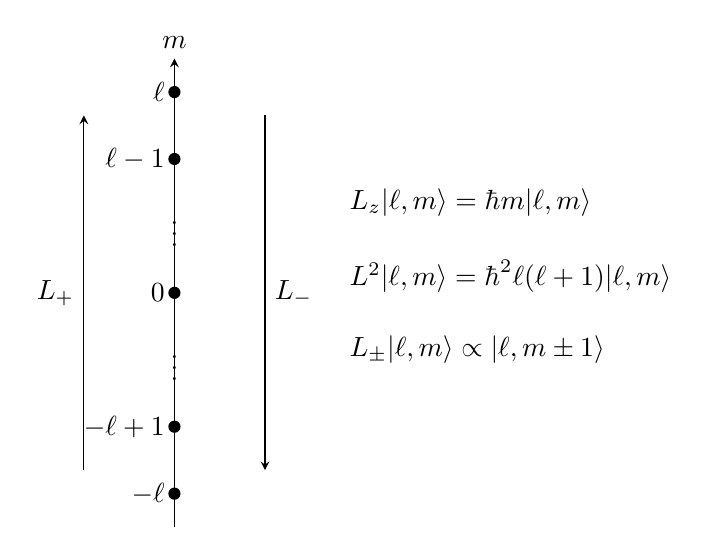
\begin{tikzpicture}[x=1cm,y=0.85cm,>=stealth]
\draw[->] (0,-3.5) -- (0,3.5) node[above] {$m$};

\fill (0,3) circle (2.2pt);
\fill (0,2) circle (2.2pt);
\fill (0,0) circle (2.2pt);
\fill (0,-2) circle (2.2pt);
\fill (0,-3) circle (2.2pt);

\node[left] at (0,3) {$\ell$};
\node[left] at (0,2) {$\ell-1$};
\node[left] at (0,0) {$0$};
\node[left] at (0,-2) {$-\ell+1$};
\node[left] at (0,-3) {$-\ell$};

\node at (0,1) {$\vdots$};
\node at (0,-1) {$\vdots$};

\draw[->] (-1.15,-2.65) -- (-1.15,2.65)
node[midway,left] {$L_+$};
\draw[->] (1.15,2.65) -- (1.15,-2.65)
node[midway,right] {$L_-$};

\node[anchor=west] at (2.1,1.35)
{$L_z|\ell,m\rangle=\hbar m|\ell,m\rangle$};
\node[anchor=west] at (2.1,0.25)
{$L^2|\ell,m\rangle=\hbar^2\ell(\ell+1)|\ell,m\rangle$};
\node[anchor=west] at (2.1,-0.85)
{$L_\pm|\ell,m\rangle\propto|\ell,m\pm1\rangle$};
\end{tikzpicture}\caption{정수 궤도 각운동량 다중항. \(L_+\)와 \(L_-\)는 \(m\)를 1만큼 바꾸며, 다중항 전체에서 \(L^2\)는 \(\hbar^2\ell(\ell+1)\)로 일정하다.}\lectureframe{00:35:53}\end{figure}

\section{중심력 문제}

다음을 생각하자.
\begin{equation}
H=\frac{\mathbf p^2}{2m}+V(r),
\end{equation}
여기서 \(V\)는 원점으로부터의 거리에만 의존한다. 회전 대칭성에 따라 각운동량은 보존된다. 고전역학에서 \(\mathbf L\)는 크기와 방향이 고정되어 있으므로 궤도는 \(\mathbf L\)에 수직인 평면 안에 머문다. 궤도는 원형일 필요도, 닫혀 있을 필요도 없다.

좌표계를 택해 이 고전적 궤도면이 \(xy\) 평면이 되도록 하고, 운동량을 방사 성분과 접선 성분으로 나누자.
\begin{equation}
\mathbf p^2=p_r^2+p_\theta^2.
\end{equation}
각운동량의 크기는
\begin{equation}
L=r p_\theta,
\end{equation}
이므로 접선 성분은 다음과 같이 쓸 수 있다.
\begin{equation}
p_\theta^2=\frac{L^2}{r^2}.
\end{equation}
해밀토니안은 다음과 같이 된다.
\begin{equation}
H=\frac{p_r^2}{2m}+\frac{L^2}{2mr^2}+V(r).
\end{equation}
\(L\)를 고정하면, 이는 방사 좌표에 대한 1차원 문제이며 유효 퍼텐셜은 다음과 같다.
\begin{equation}
V_{\mathrm{eff}}(r)=\frac{L^2}{2mr^2}+V(r).
\end{equation}
아래 칠판에는 방사 해밀토니안이 나와 있다.\footnote{출처 프레임: \texttt{\detokenize{lecture_03_frame_02.png}}, 강의 영상 시각 \(00{:}47{:}15\).}

\begin{figure}[htbp]\centering
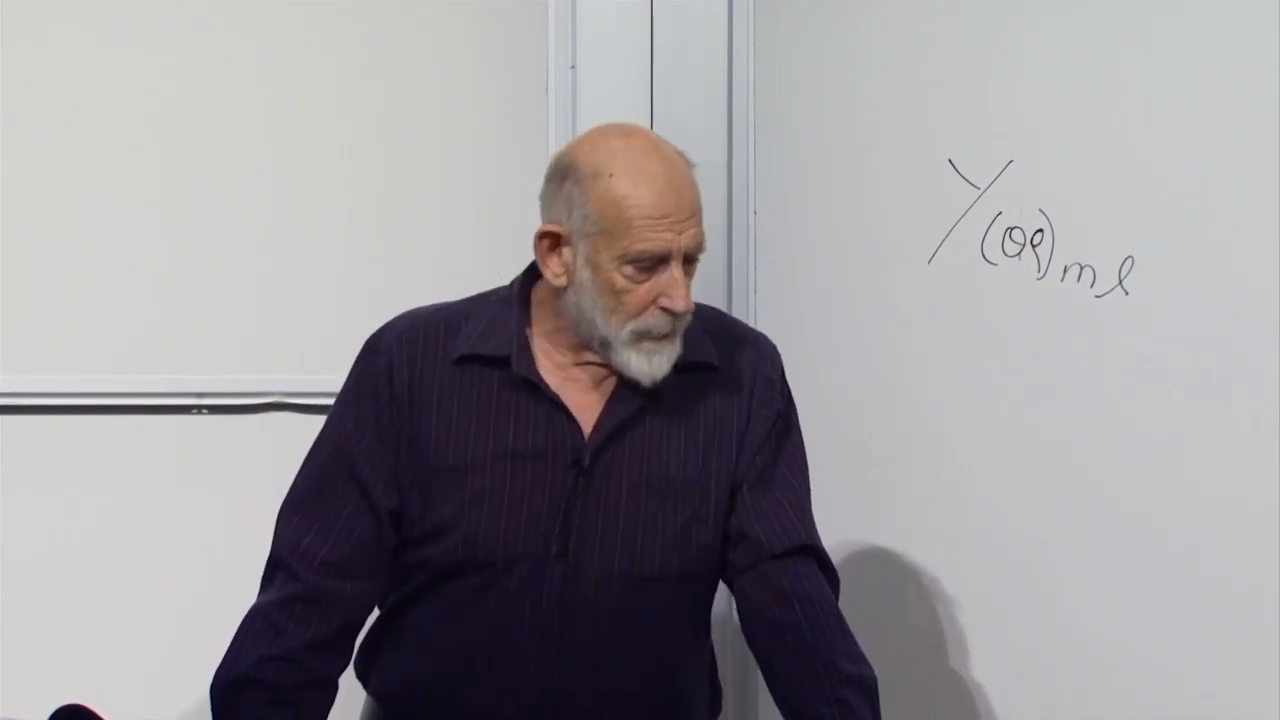
\includegraphics[width=0.9\linewidth]{lecture_03_frame_02.png}\caption{고전적 각운동량을 고정하면 방사 해밀토니안은 방사 운동에너지, 원심 항 \(L^2/(2mr^2)\), 중심 퍼텐셜 \(V(r)\)을 포함한다.}\lectureframe{00:47:15}\end{figure}

\(1/r^2\) 항은 원심 장벽이다. 입자가 원점에 가까워질수록 이 항이 커지므로, 이에 대응하는 힘은 바깥쪽을 향한다. 여기서 논의하는 쿨롱형 인력의 경우, \(L\neq0\)인 궤도는 중심에 도달하지 않고 그 주위를 돈다. \(L=0\)이면 장벽이 없다.

인력 쿨롱 퍼텐셜은
\begin{equation}
V(r)=-\frac{\kappa}{r},
\end{equation}
이다. 작은 \(r\)에서는 원심 항이 우세하고, 큰 \(r\)에서는 쿨롱 항이 더 느리게 감소하여 우세해진다. \(L\neq0\)이면 두 항의 합은 최소값을 갖는다. 최소점에서의 운동은 반지름이 일정하므로 원운동이다. 최소값보다 에너지가 높고 탈출 문턱보다 낮은 구속 운동은 최소 반지름과 최대 반지름 사이를 오간다. 쿨롱 문제에서는 이것이 타원 궤도의 방사 진동에 해당한다.

\section{축약 방사 방정식}

양자역학에서 궤도 각운동량이 확정된 상태의 각도 부분은 구면조화함수이다. 분리된 상태를 다음과 같이 쓰자.
\begin{equation}
\Psi_{n_r\ell m}(r,\theta,\phi)
=\frac{u_{n_r\ell}(r)}{r}\,
Y_{\ell m}(\theta,\phi).
\end{equation}
각 연산자 \(L^2\)의 고윳값은
\begin{equation}
L^2Y_{\ell m}
=\hbar^2\ell(\ell+1)Y_{\ell m}.
\end{equation}
이다. 고정된 양자수 쌍 \(n_r,\ell\)에 대해 \(u_{n_r\ell}(r)\)를 \(u(r)\)로 줄여 쓰자. 그러면 축약 방사 함수에 남는 방정식은 다음과 같다.
\begin{equation}
\begin{aligned}
&-\frac{\hbar^2}{2m}\frac{d^2u}{dr^2}
+\frac{\hbar^2\ell(\ell+1)}{2mr^2}u(r)\\
&\qquad+V(r)u(r)=E_{n_r\ell}\,u(r).
\end{aligned}
\end{equation}

\editorialnote{순수한 1차원 이계 미분 방정식에는 축약 방사 함수 \(u=rR\)를 사용한다. 따라서 강의 방정식에 표시된 \(\psi(r)\)는 \(u(r)\)에 해당하며, \(\Psi=R(r)Y_{\ell m}\)에 나오는 통상적인 방사 인자는 \(R=u/r\)이다. 이러한 표기법을 쓰면 \(-i\hbar\,d/dr\)를 3차원 방사 힐베르트 공간에서 그 자체로 에르미트인 방사 운동량 연산자로 취급하는 일을 피할 수 있다.}

아래 칠판에는 축약 방사 방정식이 나와 있다.\footnote{출처 프레임: \texttt{\detokenize{lecture_03_frame_03.png}}, 강의 영상 시각 \(00{:}54{:}32\).}

\begin{figure}[htbp]\centering
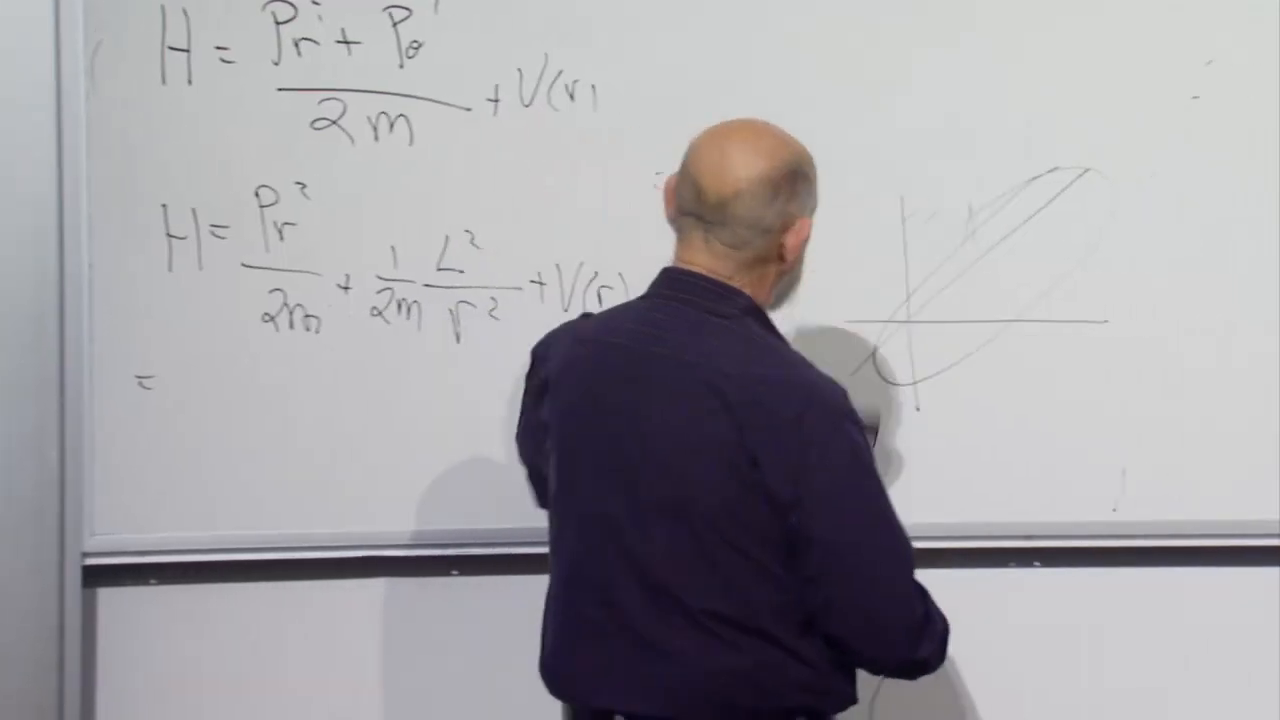
\includegraphics[width=0.9\linewidth]{lecture_03_frame_03.png}\caption{\(\ell\)를 고정하면 축약 방사 파동함수는 원심 항이 \(\ell(\ell+1)/r^2\)에 비례하는 1차원 Schr\"odinger 방정식을 만족한다.}\lectureframe{00:54:32}\end{figure}

3차원 각 구조는 매개변수 \(\ell\)에 담겨 있다. 자기 양자수 \(m\)는 방사 방정식에 나타나지 않는다.

\begin{classroomqa}\lecturetimestamp{00:55:34}\audiencequestion{\(\ell\)가 정해졌을 때, 자기 상태 \(2\ell+1\)는 모두 같은 에너지를 갖습니까?}\lecturerresponse{방사 고유상태도 고정되어 있다면 그렇습니다. \(u_{n_r\ell}\)를 하나 택할 때마다 \(m=-\ell,\ldots,\ell\)의 모든 값은 같은 에너지를 갖습니다. \(m\)가 방사 방정식에 나타나지 않기 때문입니다. 같은 \(\ell\)에서 서로 다른 방사 고유상태들은 일반적으로 에너지가 다릅니다.}\end{classroomqa}

\begin{classroomqa}\lecturetimestamp{00:56:03}\audiencequestion{왜 \(L^2\)를 \(\hbar^2\ell(\ell+1)\)로 바꿀 수 있으며, \(\ell\)은 \(m\)의 허용값과 어떤 관계가 있습니까?}\lecturerresponse{\(\ell\)은 각운동량 다중항을 표시하며 그 다중항에서 가장 큰 \(m\) 값이다. 다중항의 모든 상태는 같은 \(L^2\) 고윳값 \(\hbar^2\ell(\ell+1)\)을 가지므로, 이 고윳값을 방사 방정식에 대입한다.}\end{classroomqa}

현재 논증에는 특수 함수의 명시적 해가 필요하지 않다. 중요한 것은 해들이 어떻게 구성되는가이다.

\section{방사 마디와 에너지 준위}

\(\ell\)를 고정하면 축약 방사 방정식은 통상적인 1차원 고유값 문제가 된다. 그 속박 상태들은 내부 마디의 개수에 따라 순서가 정해진다. 가장 낮은 방사 상태에는 내부 마디가 없고, 그다음 상태에는 하나, 이어지는 상태에는 둘이 있다. 마디가 많을수록 파동함수가 더 빠르게 변하고, 파동함수가 빠르게 변할수록 운동량이 커져 운동에너지도 커진다.

\(\ell\)의 각 값은 원심 항이 \(\ell\)에 따라 달라지므로 서로 다른 방사 연산자를 정한다. 따라서 \(\ell=0,1,2,\ldots\)는 각각 별도의 방사 준위열을 이룬다. 양의 원심 항은 각운동량을 더할수록 준위를 위로 이동시킨다. 고정된 \(\ell\)에서 각 방사 고윳값에는 다음 차원의 자기 다중항이 대응한다.
\begin{equation}
2\ell+1.
\end{equation}
\(\ell=0\) 준위는 단일항이고, \(\ell=1\) 준위는 삼중항이며, \(\ell=2\) 준위는 오중항이다. 이는 회전 대칭성이 보장하는 축퇴도이다. 추가 대칭성이 있으면 \(\ell\) 값이 서로 다른 상태들도 축퇴할 수 있다.

큰 \(r\)에서 \(V(r)\to0\)을 만족하는 원자형 퍼텐셜에서는 탈출 문턱을 관례적으로 \(E=0\)으로 둔다. 음의 에너지 상태들은 이산적인 속박 스펙트럼을 이룬다. \(E=0\) 이상에서는 산란 연속 스펙트럼을 만나게 된다. 이 설명은 퍼텐셜의 큰 \(r\)에서의 거동에 달려 있으며 구속 중심 퍼텐셜에는 적용되지 않는다.

\section{쿨롱 퍼텐셜의 특별한 축퇴}

정확한 비상대론적 쿨롱 퍼텐셜에는 준위들이 추가로 정렬되는 현상이 있다. 가장 낮은 \(\ell=1\) 방사 상태는 첫 번째 들뜬 \(\ell=0\) 상태와 에너지가 같다. 다음 \(\ell=1\) 상태는 두 번째 들뜬 \(\ell=0\) 상태와 같은 에너지를 가지며, 가장 낮은 \(\ell=2\) 상태도 이들과 같은 에너지를 갖는다. 이 패턴은 더 높은 방사 및 각운동량 준위열에서도 이어진다.

\begin{classroomqa}\lecturetimestamp{01:09:57}\audiencequestion{이 추가적인 쿨롱 축퇴는 또 다른 대칭성이 있음을 뜻합니까?}\lecturerresponse{그렇습니다. 정확한 쿨롱 퍼텐셜에 존재하는 이례적인 추가 대칭성입니다. 퍼텐셜을 조금만 바꾸어도 준위 정렬은 사라지며, 그 유도 과정은 여기서 다루지 않습니다.}\end{classroomqa}

이에 따른 궤도 껍질의 축퇴도는 다음과 같다.
\begin{equation}
1,\qquad 4,\qquad 9,\qquad 16,\qquad \ldots
\end{equation}
전자 스핀은 아직 포함하지 않았다.

\begin{classroomqa}\lecturetimestamp{01:11:46}\audiencequestion{이 축퇴도는 수소 원자에 해당합니까, 아니면 이상적인 쿨롱 문제에만 해당합니까?}\lecturerresponse{수소 원자는 매우 좋은 근사로 이 관계를 만족하지만 정확히 만족하지는 않는다. 상대론적 보정과 원자핵의 유한한 크기가 이상적인 쿨롱 패턴을 흐트러뜨린다.}\end{classroomqa}

점 원자핵은 정확한 \(1/r\) 퍼텐셜을 만든다. 전하가 작은 부피에 퍼져 있는 원자핵은 전자가 그 부피 안으로 들어갈 때 약간 다른 퍼텐셜을 만들며, 이처럼 작은 차이만으로도 특별한 축퇴의 일부가 풀린다.

스핀도 빠져 있다. 전자의 두 스핀 상태를 포함하면 껍질의 상태 수는 다음과 같이 두 배가 된다.
\begin{equation}
2,\qquad 8,\qquad 18,\qquad 32,\qquad \ldots
\end{equation}
이는 더 완전한 원자 이론에서 추가적인 분열을 고려하기 전의 값이다.

\section{직교좌표 방정식 다시 보기}

방사 문제의 출발점은 3차원 시간에 무관한 Schr\"odinger 방정식이다.
\begin{equation}
\begin{aligned}
-\frac{\hbar^2}{2m}\nabla^2\Psi+V(r)\Psi&=E\Psi,\\
\nabla^2&=\frac{\partial^2}{\partial x^2}
+\frac{\partial^2}{\partial y^2}
+\frac{\partial^2}{\partial z^2},\\
r&=\sqrt{x^2+y^2+z^2}.
\end{aligned}
\end{equation}
방사 및 각좌표로 바꾸고 \(L^2\)의 고유상태를 택하자.
그러면 \(L^2\)를 \(\hbar^2\ell(\ell+1)\)로 바꾸어 편미분 방정식을 위에서 구한 통상적인 방사 방정식으로 줄일 수 있다.

\begin{classroomqa}\lecturetimestamp{01:16:42}\audiencequestion{이상적인 쿨롱 스펙트럼에서 벗어나는 정도를 이용해 원자핵의 크기를 알아낼 수 있습니까?}\lecturerresponse{이처럼 단순히 비교해서는 알 수 없습니다. 다른 보정 효과들이 훨씬 크므로 먼저 이를 고려해야 합니다. 여기서 원자핵의 크기를 언급한 이유는 점 쿨롱 퍼텐셜에서 벗어나는 한 가지 사례를 바로 들 수 있기 때문입니다.}\end{classroomqa}

\begin{classroomqa}\lecturetimestamp{01:17:09}\audiencequestion{고전 각운동량 항과 양자 각운동량 항의 주된 차이는 무엇입니까?}\lecturerresponse{고전역학에서 \(L^2\)는 보존되는 벡터 크기의 통상적인 제곱이다. 양자 궤도 다중항에서 그 고윳값은 단순히 \(\hbar^2\ell^2\)가 아니라 \(\hbar^2\ell(\ell+1)\)이다. 추가 항은 각운동량 성분들의 비가환성에서 비롯된다.}\end{classroomqa}

\begin{classroomqa}\lecturetimestamp{01:17:58}\audiencequestion{속박 상태 파동함수는 유한한 영역에만 존재합니까?}\lecturerresponse{아니다. 파동함수는 중심에서 아무리 멀리 떨어진 곳까지도 뻗어 있다. 여기서 다루는 원자 속박 상태의 경우 큰 거리에서 지수적으로 감소하므로 확률은 무시할 수 있을 만큼 작아지지만, 어떤 유한한 반지름 바깥에서 완전히 사라지지는 않는다.}\end{classroomqa}

\begin{classroomqa}\lecturetimestamp{01:18:48}\audiencequestion{\(\ell=0\)일 때 원심 퍼텐셜 우물이 사라지면 안정점은 어떻게 됩니까?}\lecturerresponse{원심 장벽과 인력의 경쟁으로 생기는 최소점이 더는 없다. 점 쿨롱 이상화에서는 고전적 운동이 특이점인 중심을 향한다. 양자역학적으로는 최저 상태가 위치를 중심에 정확히 고정하는 동시에 운동량을 0으로 가질 수 없으므로, 최저 파동함수는 유한한 공간적 퍼짐을 갖는다.}\end{classroomqa}

\editorialnote{정칙적인 중심 퍼텐셜에서는 각운동량이 0인 고전적 궤적이 원점을 지나 계속 이어질 수 있다. 반면 이상적인 점 쿨롱 퍼텐셜에서는 \(r=0\)가 충돌 특이점이므로, 고전적 궤적을 계속 이어가려면 별도의 처방이 필요하다.}

고전적 환원에서는 하나의 궤도를 한 평면 안에 두었지만, 양자 파동함수에는 같은 방법을 적용할 수 없다. 양자 궤도 상태는 3차원 공간에 퍼져 있다. 전체 각 연산자는 \(L^2=L_x^2+L_y^2+L_z^2\)이며, 그 고윳값은 3차원 결과 \(\hbar^2\ell(\ell+1)\)를 유지한다.

\begin{classroomqa}\lecturetimestamp{01:21:30}\audiencequestion{고전 궤도를 한 평면에 놓았는데도 양자 문제는 어떻게 3차원으로 남을 수 있습니까?}\lecturerresponse{보존되는 각운동량 벡터에 수직인 방향을 따라 좌표계를 잡아 한 평면에 놓은 것은 고전 궤도뿐이다. 양자 파동함수는 3차원 공간을 차지한다. 다른 각운동량 성분들도 \(L^2\)를 통해 남아 있으므로 방사 방정식에는 한 성분의 제곱만이 아니라 \(\ell(\ell+1)\)가 들어간다.}\end{classroomqa}

\begin{classroomqa}\lecturetimestamp{01:22:54}\audiencequestion{모든 양자 문제에 올림 및 내림 연산자가 있습니까?}\lecturerresponse{아니다. 이런 연산자는 특별히 유리한 경우에 나타난다. 각운동량이 그 한 예이고 조화진동자도 또 다른 예이다. 조화진동자 사례는 특히 유용하다. 안정 평형점 근처의 운동은 작은 유효 퍼텐셜 최소점 근처에서의 방사 진동을 포함해 매우 자주 조화진동으로 근사할 수 있기 때문이다.}\end{classroomqa}

이제 원자 문제는 잠시 접어 두고, 사다리 연산자로 스펙트럼을 구하는 다음 사례로 조화진동자를 살펴본다.

\section{작은 진동과 조화진동자}

안정된 평형점 근처에서는 충분히 작은 변위가 조화 운동을 일으키는 경우가 많다. 각운동량이 영이 아닌 경우의 유효 방사 퍼텐셜이 한 가지 예다. 퍼텐셜 우물의 바닥 근처에서 방사 운동은 근사적으로 조화 운동을 한다.

질량이 단위값인 일차원 진동자를 생각하자. 평형 위치로부터의 변위를 \(x\)라 하고, 용수철 상수를 \(k=\omega^2\)로 쓰자. 고전적 해밀토니안은
\begin{equation}
H=\frac{p^2}{2}+\frac{\omega^2x^2}{2}.
\end{equation}
해밀턴 방정식은 다음과 같다.
\begin{equation}
\dot{x}=\frac{\partial H}{\partial p}=p,
\qquad
\dot{p}=-\frac{\partial H}{\partial x}=-\omega^2x,
\end{equation}
따라서
\begin{equation}
\ddot{x}=-\omega^2x.
\end{equation}
그러므로 \(\omega\)는 고전적 진동수이다.

\section{인수분해와 영점 에너지}

양자역학에서는
\begin{equation}
[x,p]=i\hbar.
\end{equation}
이다. 해밀토니안이 제곱들의 합이므로 다음과 같이 인수분해할 수 있을 것으로 보인다.
\begin{align}
\frac{1}{2}(p+i\omega x)(p-i\omega x)
&=\frac{1}{2}\left(p^2+\omega^2x^2+i\omega[x,p]\right) \\
&=\frac{1}{2}\left(p^2+\omega^2x^2-\hbar\omega\right).
\end{align}
따라서
\begin{equation}
H=\frac{1}{2}(p+i\omega x)(p-i\omega x)
+\frac{1}{2}\hbar\omega.
\end{equation}
이다. 더해지는 항 \(\hbar\omega/2\)은 영점 에너지이다.

고전적으로는 \(x=p=0\)일 때 에너지가 최솟값을 갖는다. 양자역학적으로는 위치와 운동량이 모두 영으로 정확히 정해진 상태는 있을 수 없다. 또한 두 항 \(p^2/2\)와 \(\omega^2x^2/2\)은 양수이므로 서로 상쇄될 수 없다. 따라서 바닥 상태 에너지가 영이 아닌 것은 불가피하다.

사다리 계산에서는 공통으로 더해지는 상수항을 잠시 빼 두었다가 마지막에 복원해도 된다.

\begin{classroomqa}\lecturetimestamp{01:36:10}\audiencequestion{영점 항의 양의 부호가 추가로 알려 주는 것이 있습니까?}\lecturerresponse{진동자 해밀토니안은 양의 연산자이다. 양의 제곱들의 합이므로 에너지는 음수가 될 수 없다.}\end{classroomqa}

\section{진동자의 사다리}

무차원 연산자를 도입하자.\footnote{\(01{:}37\)--\(01{:}42\)계산 과정에서는 \(\hbar=1\)를 사용한다. 이 정규화된 정의에서는 \(\hbar\) 인자를 복원하여 \(A_\pm\)가 무차원이고 교환자가 1이 되도록 한다.}
\begin{equation}
A_+=\frac{p+i\omega x}{\sqrt{2\hbar\omega}},
\qquad
A_-=\frac{p-i\omega x}{\sqrt{2\hbar\omega}}.
\end{equation}
이들은 서로 에르미트 켤레이다.
\begin{equation}
A_+^\dagger=A_-.
\end{equation}
교환자는
\begin{align}
[A_-,A_+]
&=\frac{1}{2\hbar\omega}
\left([p,i\omega x]+[-i\omega x,p]\right) \\
&=1.
\end{align}
이다.

다음을 정의하자.
\begin{equation}
N=A_+A_-.
\end{equation}
그러면 해밀토니안은
\begin{equation}
H=\hbar\omega\left(N+\frac{1}{2}\right).
\end{equation}
이다. 따라서 에너지 스펙트럼을 구하는 문제는 \(N\)의 고윳값을 구하는 문제로 바뀐다.

다음과 같이 두자.
\begin{equation}
N|n\rangle=n|n\rangle.
\end{equation}
\(N\)와의 교환자는 다음과 같다.\footnote{\(01{:}45{:}37\)--\(01{:}48{:}10\)에서의 중간 계산은 주어진 관계식 \(N=A_+A_-\)와 \([A_-,A_+]=1\)에서 직접 재구성할 수 있다.}
\begin{align}
[N,A_+]
&=A_+[A_-,A_+]=A_+, \\
[N,A_-]
&=[A_+,A_-]A_-=-A_-.
\end{align}
따라서
\begin{align}
N\bigl(A_+|n\rangle\bigr)
&=(n+1)A_+|n\rangle, \\
N\bigl(A_-|n\rangle\bigr)
&=(n-1)A_-|n\rangle.
\end{align}
결과 벡터가 영이 아닌 경우, \(A_+\)는 \(N\)의 고윳값을 한 단위 높이고 \(A_-\)는 한 단위 낮춘다.

연산자 \(N\)는 음이 아닌 값을 갖는다.
\begin{equation}
\langle\psi|N|\psi\rangle
=\langle\psi|A_+A_-|\psi\rangle
=\|A_-|\psi\rangle\|^2
\geq0.
\end{equation}
따라서 내림 과정은 음의 고윳값으로 이어질 수 없다. 최하단 상태 \(|b\rangle\)에서는 과정이 끝나야 한다.
\begin{equation}
A_-|b\rangle=0.
\end{equation}

정규화된 고유상태에서는 사다리 계수가 상태의 노름으로 정해진다.
\begin{align}
\|A_-|n\rangle\|^2
&=\langle n|A_+A_-|n\rangle=n, \\
\|A_+|n\rangle\|^2
&=\langle n|A_-A_+|n\rangle=n+1.
\end{align}
따라서 위상은 다음과 같이 선택할 수 있다.
\begin{equation}
A_-|n\rangle=\sqrt{n}\,|n-1\rangle,
\qquad
A_+|n\rangle=\sqrt{n+1}\,|n+1\rangle.
\end{equation}

\begin{classroomqa}\lecturetimestamp{01:52:42}\audiencequestion{\(A_-\)가 상태를 낮추고 \(A_+\)가 다시 올리면, \(A_+A_-\)는 어떻게 고윳값 \(n\)를 만들어 냅니까?}\lecturerresponse{사다리 연산의 작용에는 정규화 인자가 포함된다. 먼저 \(A_-\)를 작용시키면 \(\sqrt n\)가 곱해지고, 그 결과 상태에 \(A_+\)를 작용시키면 다시 \(\sqrt n\)가 곱해진다. 두 인자의 곱은 \(n\)이다.}\end{classroomqa}

실제로,
\begin{equation}
A_+A_-|n\rangle
=\sqrt n\,A_+|n-1\rangle
=n|n\rangle.
\end{equation}

\begin{classroomqa}\lecturetimestamp{01:55:52}\audiencequestion{\(N\)의 최저 고윳값은 반드시 0이어야 합니까, 아니면 양수일 수도 있습니까?}\lecturerresponse{반드시 0이어야 하며, \(N\)의 스펙트럼은 음이 아닌 정수들로 이루어진다. 아직 이 끝점에 대한 증명은 제시하지 않았다.}\end{classroomqa}

\editorialnote{\(|b\rangle\)를 최저 상태라고 하자. 낮춤 연산은 반드시 끝나야 하므로 \(A_-|b\rangle=0\)이다. 따라서 곧바로 \(N|b\rangle=A_+A_-|b\rangle=0\)를 얻으며, 그러므로 \(N\)의 최저 고윳값은 0이다.}

이 최저 상태에서 시작해 \(A_+\)를 적용하면
\begin{equation}
n=0,1,2,\ldots.
\end{equation}
더해 둔 영점 항을 복원하면 진동자 에너지는 다음과 같다.
\begin{equation}
E_n=\hbar\omega\left(n+\frac{1}{2}\right),
\qquad n=0,1,2,\ldots.
\end{equation}

진동자 대수는 더 발전시켜 다른 양자 문제를 푸는 데도 사용한다.
